\documentclass[12pt]{article}

\usepackage{indentfirst}
\usepackage{hyperref}
\usepackage{graphicx}
\usepackage[margin=1in]{geometry}
\usepackage{setspace}
\usepackage{amsfonts}

\usepackage[L7x,T1]{fontenc}
\usepackage[utf8]{inputenc}
\usepackage[lithuanian,english]{babel}

\graphicspath{ {./figures/} }

\setstretch{1.5}

\thispagestyle{empty}

\newcommand{\specialcell}[2][c]{%
  \begin{tabular}[#1]{@{}c@{}}#2\end{tabular}}

\begin{document}
	\begin{center}

	    \vspace*{1cm}
	    \Large
	    Vilnius University

		Mathematics and Informatics Faculty

		Institute of Informatics 

		Bioinformatics study program
	    
        \vspace*{2cm}
        \Large
		\textbf{Protein thermostability prediction using 
		sequence representations from protein 
		language models}

	\end{center}

	\begin{flushright}

		\vspace*{2cm}
        \large
        Author: Ieva Pudžiuvelytė

        Supervisor: Kliment Olechnovič, PhD 
        
	\end{flushright}

	\begin{center}
		\vspace*{4cm}
        \large
        Course work project
        
        \vspace*{2cm}
        \large
        Vilnius, 2023
	\end{center}
	
	\newpage

	\tableofcontents

	\newpage
	
	\section{Introduction}

	This work is a continuation of the previous work - the model 
	that performed binary classification into thermostability 
	classes. The model, which was a single-layer perceptron (SLP), 
    took protein language model's ESM-1b \cite{rives2021biological} 
	protein embeddings as input 
	and provided prediction for each protein, how likely it 
	belongs to the thermostable class.

    The classes of thermostability were defined the following 
    way: proteins that were considered as stable in lower that 
    65 degrees of Celsius were labelled with '0' and the remaining
	proteins were labelled with '1'. 
    
    The classifier was trained on the data set 
	\cite{engqvist_martin_karl_magnus_2018_1175609} that contained 
	proteome identifiers, which were used 
    to collect proteins. The data set also contained information 
	about organism's growth temperature, therefore proteins that 
	belonged to a particular proteome were labelled accordingly. 

    Nevertheless the classifier showed promising results, yet an
    important downside of the developed method was emphasized -
    since ESM-1b embeddings generation was limited by the size 
    of the protein, the model could not provide predictions for 
    proteins that were longer than 1022 amino acids. For this 
    reason, it was decided to try ProtTrans 
	\cite{elnaggar2020prottrans} embeddings as an 
    input for the classification model.

    Furthermore, it was interesting to exploit not only mean 
    embeddings, but also to check whether a different 
    connection of per residue embeddings would improve the 
    performance of the classification model.

    In addition to these fixed tasks, another objective of 
	this work was to examine whether other variants of model
	architectures would improve the classifier's results.

	The results of this analysis showed that the best embeddings 
	representations to use until the final training data set is 
	established are ProtTrans mean and octiles representations. 
	Additionally, it was observed that the most suitable model 
	of those that were tested in this work for protein classification in
	terms of thermostability is the feed-forward 
	neural network with two hidden layers.

    The results of this work contribute to the further development of
	the final method for binary protein classification into 
	thermostability classes.

	\normalsize
	
	\newpage

	\section{Materials and methods}

	\subsection{Protein language models}

	Protein language models are transformer models trained on protein sequences.
	The transformer is a model, which is made of encoder-decoder architecture 
	that relies entirely on self-attention \cite{vaswani2017attention}. 
	Attention in deep learning is a mechanism that finds the most influential
	factors in the data and focuses on them when it processes the input. 
	Particularly, self-attention is a component of the network's architecture
	that quantifies dependencies between the input elements.

	The encoder part provides continuous representations of the input composed 
	of sequences of symbols, meanwhile the decoder part generates output for each 
	symbol in the input sequence. For this principle of architecture, transformers
	can be trained in an unsupervised fashion and be applied to natural language
	processing (NLP) tasks at which they produce state-of-the-art 
	results \cite{vig2019analyzing}.

	Since amino acid sequences can be considered as a particular language, 
	transformer architectures were applied to solve tasks related to protein 
	biology or molecule modelling \textit{in silico}. Attention mechanisms in 
	models of transformer architecture, taking BERT-like model as an example 
	\cite{vig2020bertology}, are capable to capture the folding structure, 
	binding sites, and complex biophysical properties of proteins.

	This work continues to exploit the transfer learning by taking 
	protein representations from the last layer of protein language 
	models and passing them as input to the classification 
	model (Figure \ref{figure:EmbeddingsUsageScheme}).

	\begin{figure}[h!]
		\centering
		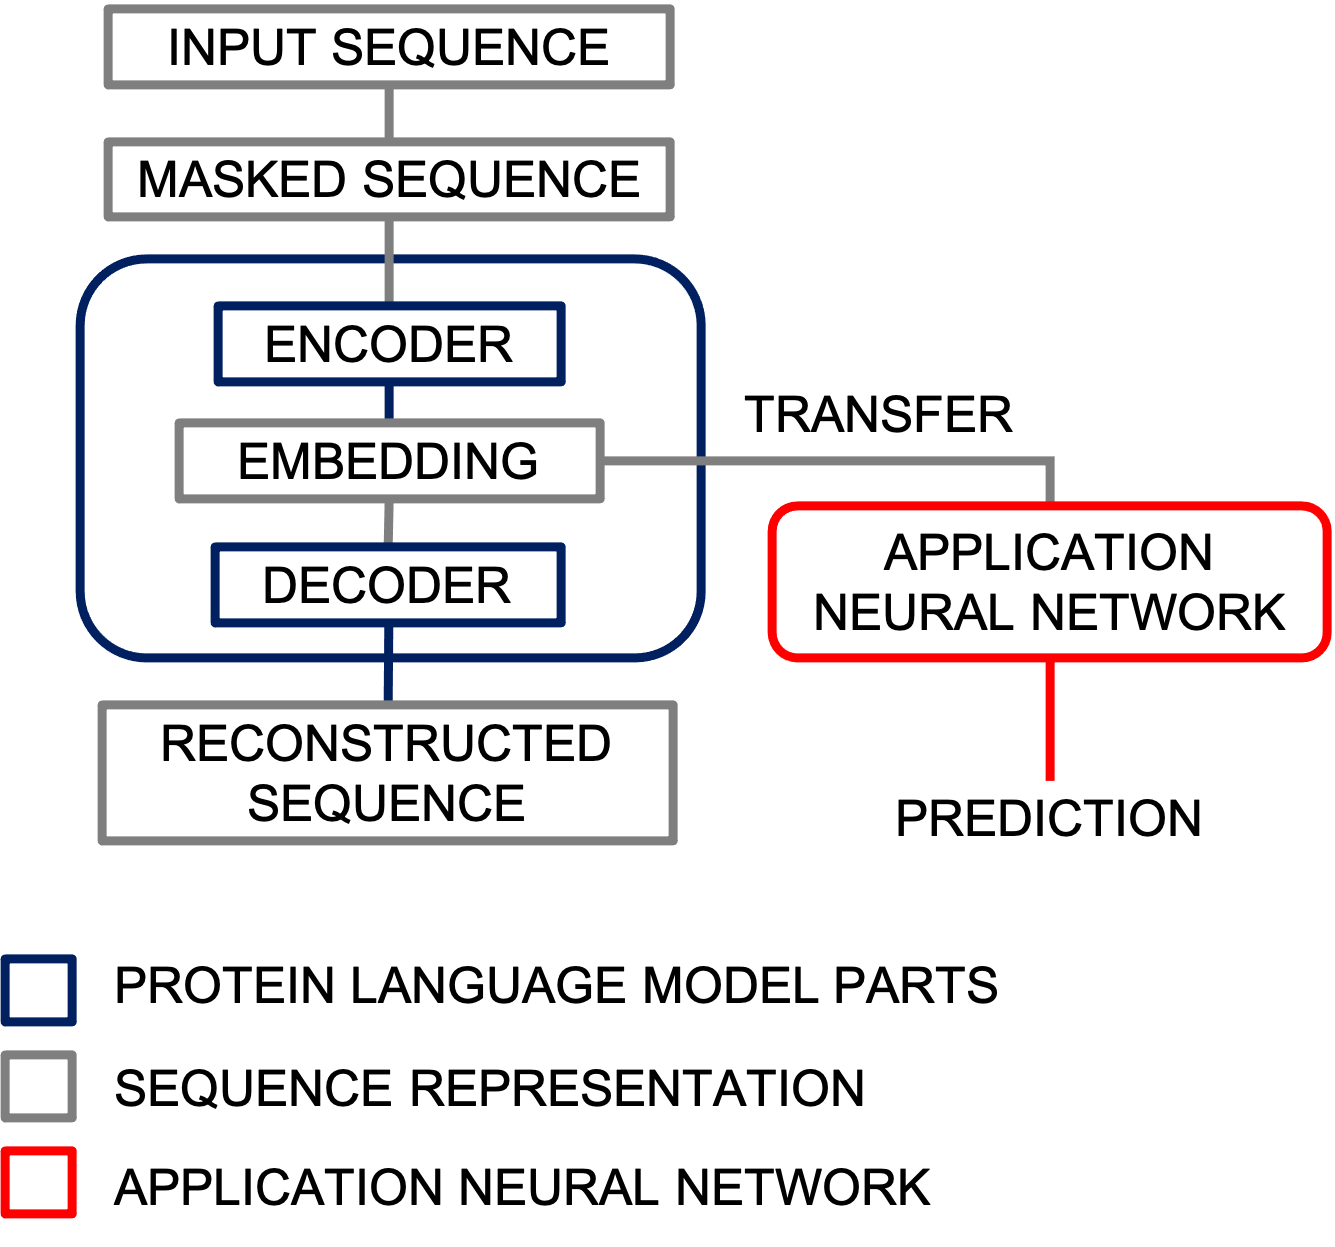
\includegraphics[scale=0.4]{scheme.png}

		\caption{The scheme of embeddings from protein language model usage in the 
		application neural network model}
		\label{figure:EmbeddingsUsageScheme}
	\end{figure}

	\subsection{ESM-1b embeddings}

	Due to the novelty of embeddings, a considerably good performance of
	protein language models, and a recently emerged availability of embeddings,
	it was decided to develop a neural network model that would take protein
	embeddings as input and give the thermostability class
	label as output.

	ESM-1b is one of evolutionary scale models trained by Facebook Research 
	\cite{rives2021biological}. The model has 33 layers and 650 million parameters. 
	The model was trained in an 
	unsupervised fashion on 
	\href{ftp://ftp.uniprot.org/pub/databases/uniprot/uniref/uniref50}{UniRef50 data set}
	(accessed March 28, 2018)\cite{suzek2015uniref}. In order 
	to ensure
	determinism in the validation set, authors removed protein sequences that
	were longer than 1024 amino acids. 

	The authors made a script to extract model's embeddings available in the 
	\href{https://github.com/facebookresearch/esm}{repository "Evolutionary Scale Modelling"}.
	The script allows to choose 
	from which model and layer embeddings will be taken, what embeddings 
	(mean, per amino acid, or beginning of the sequence token) to keep. In the
	result of using the script, a 1280 dimensional vector for each protein is 
	generated.
	
	The fact that sequences longer than 1024 amino acids were removed from the 
	validation data set for ESM-1b model's training implies to the limitation of 
	model's embeddings, which cannot be generated for sequences longer than 
	1024 amino acids.

	\subsection{ProtTrans embeddings}

	ProtTrans \cite{elnaggar2020prottrans} is a collection 
	of protein language models 
	(LMs) that were trained to learn information about 
	proteins and encode it. ProtTrans embeddings are vector 
	representations taken from the last hidden state of 
	the protein LM. 

	In particular, ProtT5-XL model was used in this work and 
	exactly this model will be referred to by the name of 
	'ProtTrans'. Overall, this model has 24 layers. In particular, 
	the size of the hidden layer, from which the 
	embedding is taken, is 1024. This model was trained on 
	BFD-100 data set 
	and fine-tuned on UniRef50. Since ProtT5-XL model was 
	considered by the 
	authors as the best-performing model, it was chosen to be 
	applied in this work. Additionally, this model 
	does not have 
	positional encoding limit, which means that there is no 
	limitation for the protein's size to generate its embedding. 

	Furthermore, according to the article, in which ProtTrans
	project was published, ProtT5-XL models (trained on BFD-100 
	and UniRef50 data sets separately) 
	outperformed ESM-1b \cite{rives2021biological} model.

	\subsection{Training and evaluation data set}

	In this work two types of data sets were used: for the analysis of 
	principal components' the data set was directly inherited from the previous 
	work: a subset of the data set of 21498 
	annotated organisms \cite{engqvist_martin_karl_magnus_2018_1175609}, which 
	is identified as '003' data set, and the filtered version of it.
	
	'003' was constructed to be balanced and 
	that a single taxonomy identifier from the collection of annotated organisms 
	would be present only in either training, validation, or testing subset. 
	Proportions that were chosen to divide '003' data set were 70\%, 
	15\%, and 15\% for training, validation, and testing sets respectively. 
	Additionally, since this data set 
	was first created with an intention to test the classifier that used ESM-1b 
	embeddings as input, all sequences included in '003' are no longer 
	than 1022 amino acids.
	
	Although the analysis of other representations was carried 
	out using '003' data set that was filtered from identically matching 
	sequences to get more accurate evaluations.

	\begin{table}[h!]
		\caption{Number of sequences with embeddings before and after 
		filtering the data set}
		\vspace{0.2cm}
		\centering
		\begin{tabular}{ | c | c c | }
			\hline 
			Subset & Original & After filtering \\
			\hline 
			Training & 284309 & 283360 \\
			Validation & 65156 & 63158 \\
			Testing & 73662 & 73308 \\
			\hline    
		\end{tabular}
		\label{table:numberEmbeddings}
	\end{table}

	\begin{table}[h!]
		\caption{Number of sequences with embeddings in each class 
		before and after filtering the data set}
		\vspace{0.2cm}
		\centering
		\begin{tabular}{ | c | c c | }
			\hline 
			Class & Original & After filtering \\
			\hline 
			0 & 216595 & 212129 \\
			1 & 212729 & 207697 \\
			\hline    
		\end{tabular}
		\label{table:numberEmbeddingsClasses}
	\end{table}

	\newpage

	\subsection{Components' correlation analysis}

	As a consequence of the former work, this thesis includes 
	analysis of ProtTrans protein language model's mean embeddings 
	usage in protein classification. Yet also, since one of the 
	tasks of this work (given in the
	section \ref{analysedRepresentations}) is to try joined ESM-1b and ProtTrans 
	representations as an input to the thermostability classification 
	model, the correlation coefficients between the components of mean 
	embeddings were analysed.

	For this analysis only a small subset of '003' data set was chosen
	(Table \ref{table:numberEmbeddingsCorrAnalysis}).

	\begin{table}[h!]
		\caption{Number of sequences with embeddings used for correlation analysis}
		\vspace{0.2cm}
		\centering
		\begin{tabular}{ | c  c | c | }
			\hline 
			Class '0' & Class '1' & Overall \\
			\hline 
			6096 & 6150 & 12246 \\
			\hline
		\end{tabular}
		\label{table:numberEmbeddingsCorrAnalysis}
	\end{table}

	Besides the original mean embeddings, principal components that explain 95\% 
	of variance
	of ESM-1b and ProtTrans
	mean embeddings (527 and 443 components for each language model 
	respectively) were retrieved and taken for the correlation 
	analysis.

	\subsection{Analysed representations}
	\label{analysedRepresentations}
	
	Both protein language models - ESM-1b and 
	ProtTrans - provide 
	per token or per residue representations - each 
	amino acid of the protein gets a 1280 or 1024-dimensional vector from
	ESM-1b or ProtTrans model respectively. Therefore, each protein is 
	originally represented by the ${m \times n}$ matrix, 
	where ${m}$ is the number of dimensions of the chosen type of embedding
	and ${n}$ is the number of amino acids that compose the protein. 
	These representations are processed to get vectors with the same 
	dimension 
	for each protein in the data set. 
	
	Additionally, it was decided to analyse whether a normalisation of 
	embeddings determines better results. Both ESM-1b and ProtTrans 
	embeddings were normalised using the standard score principle for 
	each element of the embedding (Eq. \ref{normalisationStandardScore}). 
	The procedure was executed for both 
	types of protein language models' embeddings separately. The training
	set's embeddings were used to calculate means and standard deviations 
	of each component, which resulted in 1024 and 1280 means 
	and standard deviations for ProtTrans and ESM-1b cases respectively.

	\begin{equation}
		z_i = \frac{x_i-\mu_i}{\sigma_i},\ where\ i\in\{1, 2, ..., m\}\subset \mathbb{N},\ where\ m\in \{1024, 1280\} 
		\label{normalisationStandardScore}
	\end{equation}

	The normalised mean embeddings of protein language models were 
	used separately and joined together.
	
	Eventually, the representations 
	included in the analysis were:

	\begin{enumerate}
		\item Mean ESM-1b and ProtTrans 
		\item Joined mean ESM-1b and ProtTrans
		\item Normalised mean ESM-1b and ProtTrans
		\item Joined normalised mean ESM-1b and ProtTrans
		\item Median ESM-1b and ProtTrans
		\item Minimum, median, and maximum ESM-1b and ProtTrans
		\item Quantiles (including minimum and maximum) ESM-1b and ProtTrans
		\item Quantiles (including minimum and maximum) and mean ESM-1b and ProtTrans
		\item Octiles (including minimum and maximum) ESM-1b and ProtTrans
	\end{enumerate}

	\begin{table}[h!]
		\caption{Sizes of the analysed representations' vectors}
		\vspace{0.2cm}
		\centering
		\begin{tabular}{ | c | c c | }
			\hline 
			Representation & ESM-1b & ProtTrans \\
			\hline 
			Mean & 1280 & 1024 \\
			Joined mean & \multicolumn{2}{c|}{2304} \\
			Median & 1280 & 1024 \\
			Minimum, median, maximum & 3840 & 3072 \\
			Quantiles & 6400 & 5120 \\
			Quantiles and mean & 7680 & 6144 \\
			Octiles & 11520 & 9216 \\
			\hline    
		\end{tabular}
		\label{table:vectorsDimensions}
	\end{table}

	\newpage

	\subsection{Analysed architectures}

	All representations that were described
	in the previous section were taken as input for the baseline
	single-layer perceptron models, although another important part 
	of this work was to explore several different 
	model architectures. 

	Architectures that were chosen to run experiments with 
	had one or two hidden layers. The sizes of hidden layers 
	were chosen to be original embeddings size divided 
	by several multiples of 2 (Tables \ref{table:modelArchitecturesESM} 
	and \ref{table:modelArchitecturesPT}, 
	Figures \ref{figure:architecture1HL} and \ref{figure:architecture2HL}). That is, since the 
	size of the ESM-1b embedding is 1280, there were 
	models defined with one hidden layer of size 640, 320, or 160 
	that take ESM-1b embeddings as input. For models with two 
	hidden layers, sizes of hidden layers were assigned by 
	combining two sequential sizes received from division. 
	Analogously, the same operation was done for models adjusted 
	for ProtTrans.

	In order to compare the SLP results with the results of new 
	architectures, for all models 
	batch size equal to 24, and Adam optimiser \cite{kingma2014adam} 
	with learning rate of 0.0001 were chosen. Activation function was 
	chosen to be \href{https://pytorch.org/docs/stable/generated/torch.nn.Sigmoid.html}{sigmoid}
	(coinciding with the previous work) and loss function - 
	\href{https://pytorch.org/docs/stable/generated/torch.nn.CrossEntropyLoss.html}{cross entropy loss}
	adjusted for binary classification case (the main reason for it was to unify loss functions between 
	binary and multiclass classification, which was put to the test out of this work's scope). 
	The later change determined  insignificantly different prediction values.

	\begin{table}[h!]
		\caption{Models that were tested with ESM-1b embeddings input}
		\vspace{0.2cm}
		\centering
		\begin{tabular}{ | c | c c | }
			\hline 
			Model & Number of hidden layers & Size of hidden layers \\
			\hline 
			C2H2\_h640-320 & 2 & 640, 320 \\
			C2H2\_h320-160 & 2 & 320, 160 \\
			C2H1\_h640 & 1 & 640 \\
			C2H1\_h320 & 1 & 320 \\
			C2H1\_h160 & 1 & 160 \\
			SLP\_ESM-1b & 0 & - \\
			\hline    
		\end{tabular}
		\label{table:modelArchitecturesESM}
	\end{table}

	\begin{table}[h!]
		\caption{Models that were tested with ProtTrans embeddings input}
		\vspace{0.2cm}
		\centering
		\begin{tabular}{ | c | c c | }
			\hline 
			Model & Number of hidden layers & Size of hidden layers \\
			\hline 
			C2H2\_h512-256 & 2 & 512, 256 \\
			C2H2\_h256-128 & 2 & 256, 128 \\
			C2H1\_h512 & 1 & 512 \\
			C2H1\_h256 & 1 & 256 \\
			C2H1\_h128 & 1 & 128 \\
			SLP\_ProtTrans & 0 & - \\
			\hline    
		\end{tabular}
		\label{table:modelArchitecturesPT}
	\end{table}

	\newpage

	\begin{figure}[h!]
		\centering
		
\includegraphics[scale=0.6]{architecture_0hl.png}

		\caption{A scheme of a single layer perceptron classification model}
		\label{figure:architecture0HL}
	\end{figure}

	\begin{figure}[h!]
		\centering
		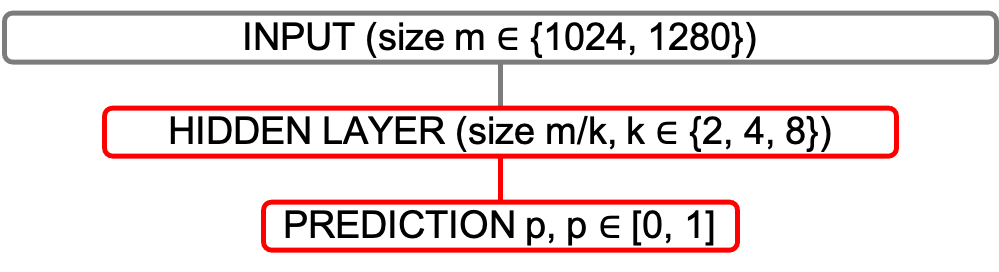
\includegraphics[scale=0.6]{architecture_1hl.png}

		\caption{A scheme of classification model with one hidden layer}
		\label{figure:architecture1HL}
	\end{figure}

	\begin{figure}[h!]
		\centering
		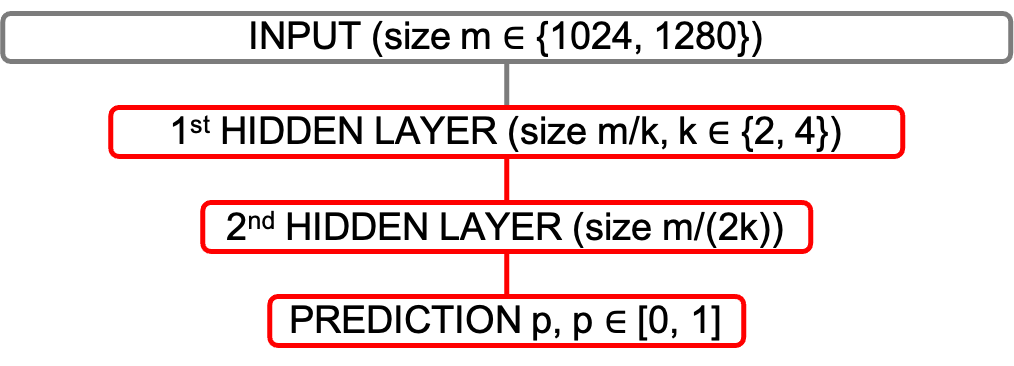
\includegraphics[scale=0.6]{architecture_2hl.png}

		\caption{A scheme of classification model with two hidden layers}
		\label{figure:architecture2HL}
	\end{figure}

	\newpage

	\section{Results}

	\subsection{Correlation analysis of embeddings' components}

	The results of the analysis showed that there are five ESM-1b
	embeddings' components that have absolute correlation coefficients 
	higher than 0.5 with more than 10 ProtTrans embeddings' components  
	(Figure \ref{figure:highCorrelationComponents}). However, overall the 
	majority of components' pairs had correlation coefficients close to zero 
	(Figure \ref{figure:correlationComponentsHisto}).

	\begin{figure}[h!]
		\centering
		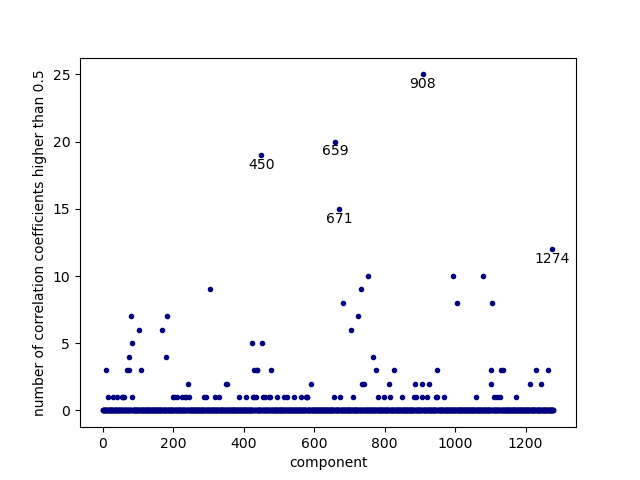
\includegraphics[scale=0.85]{validation_small_set_2_joined_correlation_high_corr.png}

		\caption{Plot of ESM-1b components that have got high absolute correlation 
		coefficients with ProtTrans components}
		\label{figure:highCorrelationComponents}
	\end{figure}

	\newpage

	\begin{figure}[h!]
		\centering
		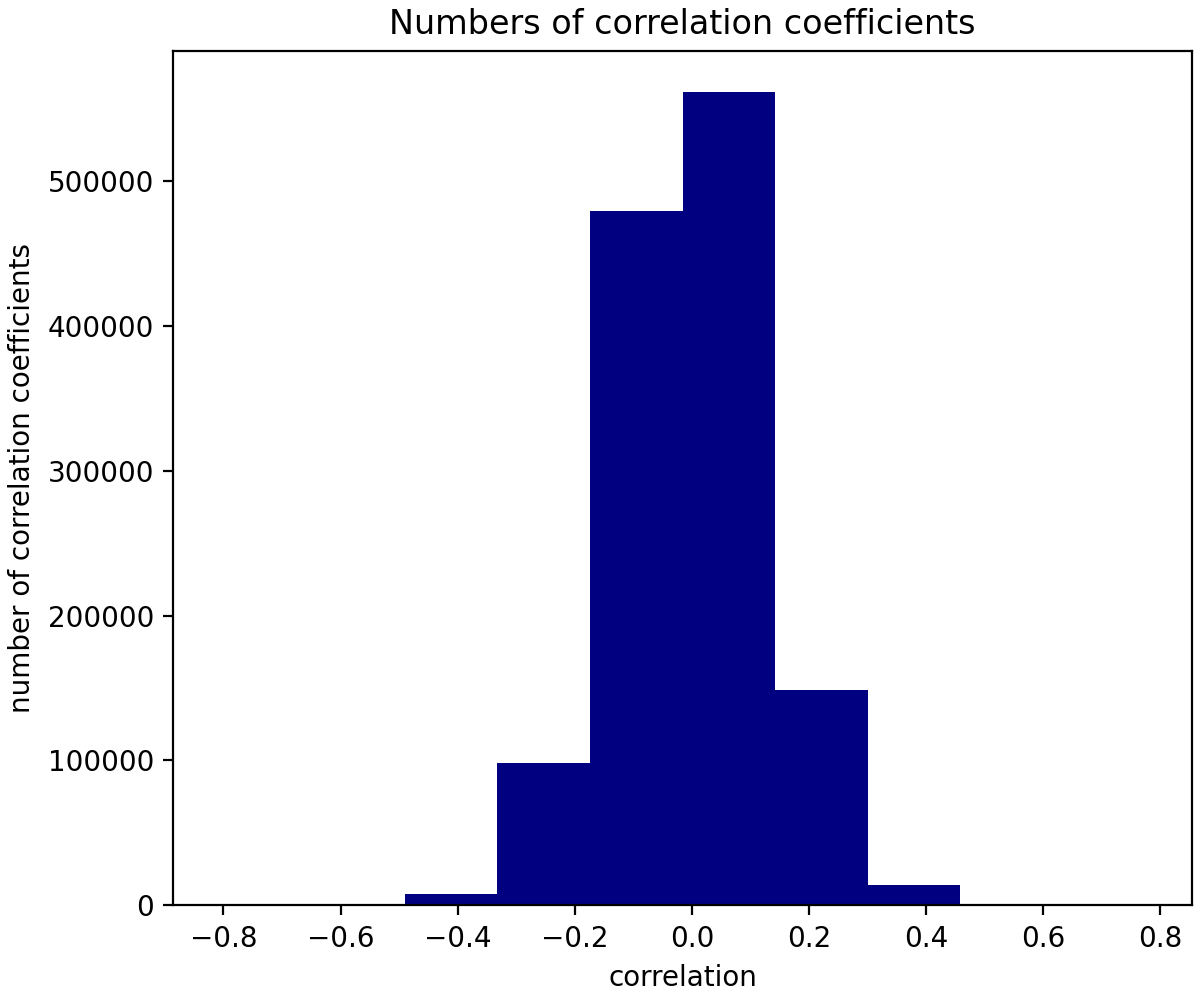
\includegraphics[scale=0.85]{validation_small_set_2_joined_correlation_hist.png}

		\caption{Histogram of correlation coefficients between ESM-1b 
		and ProtTrans components}
		\label{figure:correlationComponentsHisto}
	\end{figure}

	\newpage

	The plot that visualises absolute maximum correlation coefficients between 
	pairs of components has a curve (Figure \ref{figure:correlationComponentsMaxAndMean}). 
	that shows raw coefficient correlation values - there are peaks 
	at ESM-1b positions that correspond with positions that have the 
	biggest number of high (absolute value above 0.5) correlation coefficients
	(Figure \ref{figure:highCorrelationComponents}). Therefore, it can 
	be concluded that there are no intervals of ESM-1b components that have 
	a considerably high correlation with ProtTrans components.

	The observations that can be made from the plot of averaged correlation 
	coefficients (Figure \ref{figure:correlationComponentsMaxAndMean}) do not change the 
	overview of the correlation between 
	ESM-1b and ProtTrans components - the overall mean of correlation coefficients 
	is around 0.1.

	\begin{figure}
		\centering
		\begin{tabular}{@{}c@{}}
			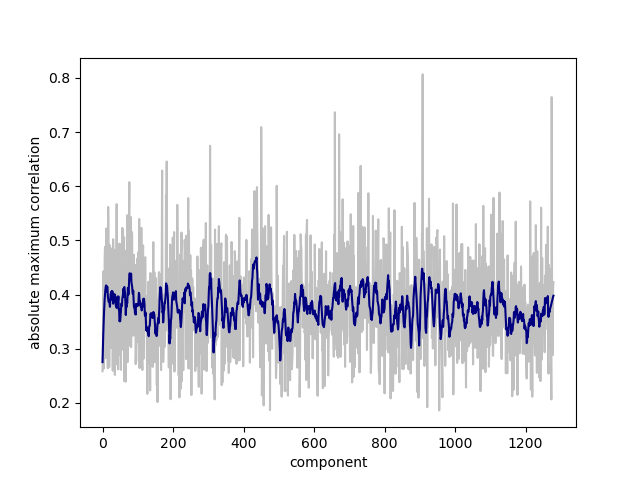
\includegraphics[scale=0.85]{validation_small_set_2_joined_correlation_max.png}
		\end{tabular}

		\begin{tabular}{@{}c@{}}
			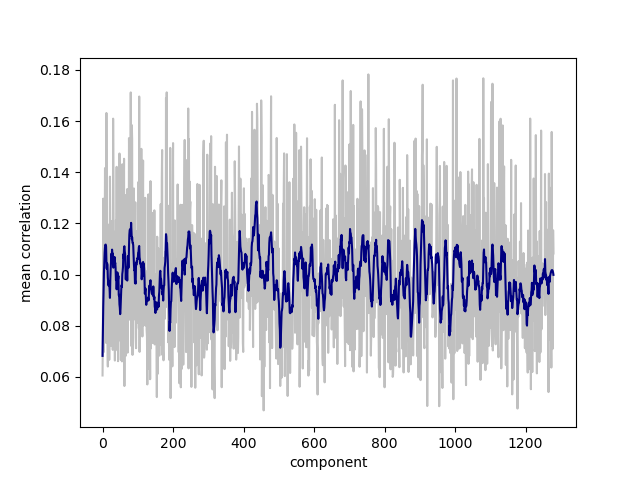
\includegraphics[scale=0.85]{validation_small_set_2_joined_correlation_mean.png}
		
		\end{tabular}
		
		\caption{Plots of ESM-1b components' maximum and mean absolute correlation coefficients 
		with ProtTrans components}\label{figure:correlationComponentsMaxAndMean}
	\end{figure}

	\newpage

	Additionally, it was attempted to analyse correlation coefficients between 
	embeddings' principal components that explain 95 percent of data variation.

	The analogous scatter plot of the number of absolute correlation 
	coefficients higher than 0.5 was drawn for principal components.
	The analysis implied that there are only few high correlation coefficients 
	between components' pairs overall.

	The curve of absolute maximum correlation coefficients shows 
	that there is a trend of correlation coefficients to decrease 
	as the index of ESM-1b component is increasing 
	(Figure \ref{figure:correlationComponentsMaxAndMeanPC95}). The following 
	plot of mean correlation coefficients 
	(Figure \ref{figure:correlationComponentsMaxAndMeanPC95}) supports the 
	statement that high maximum values of absolute correlation 
	coefficients are not dominating 
	because the mean correlation is very small between the pairs.

	\begin{figure}
		\centering
		\begin{tabular}{@{}c@{}}
			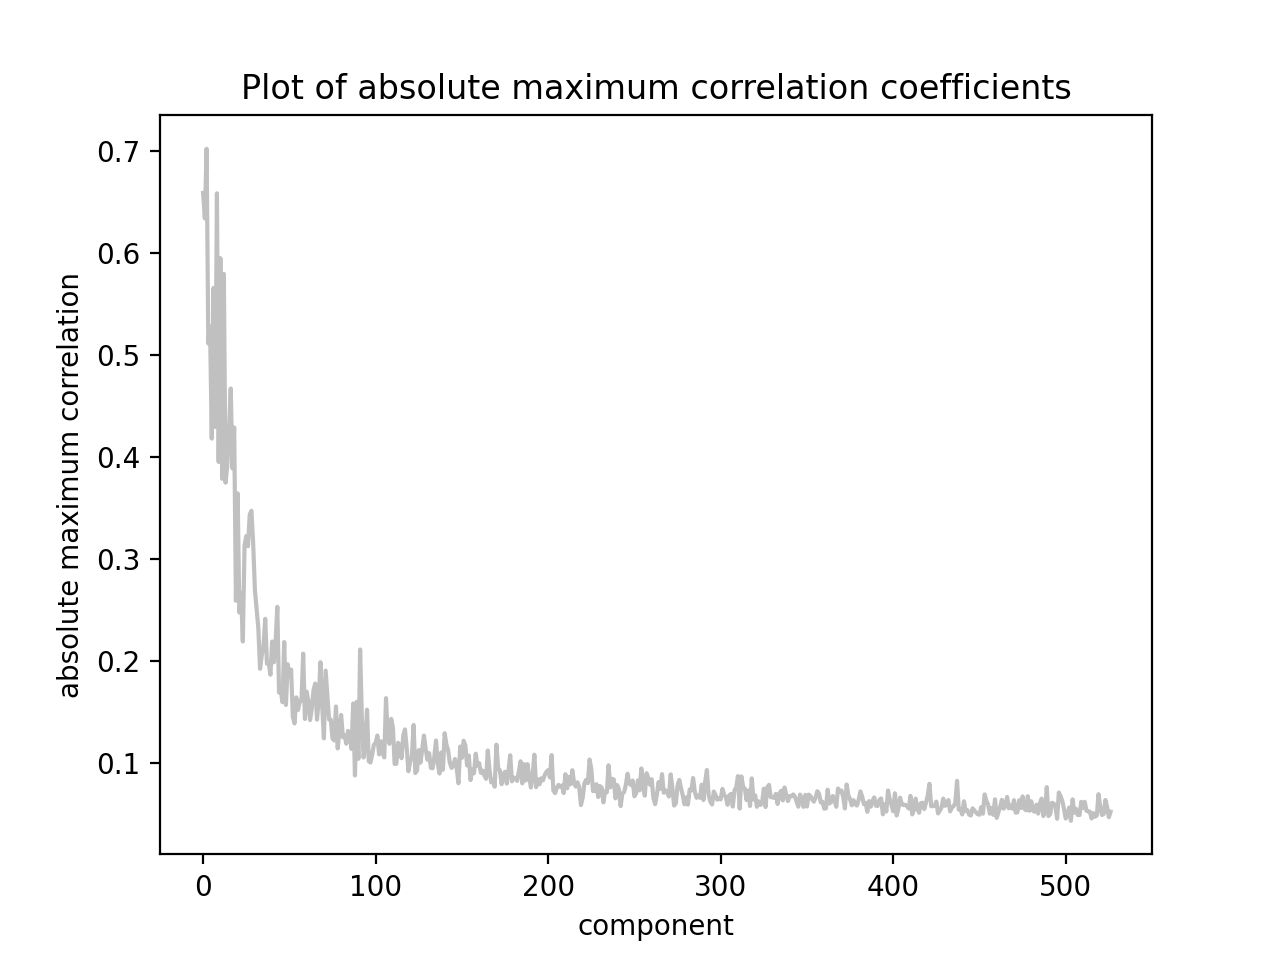
\includegraphics[scale=0.85]{validation_small_set_2_joined_PC_95_correlation_max.png}
		\end{tabular}

		\begin{tabular}{@{}c@{}}
			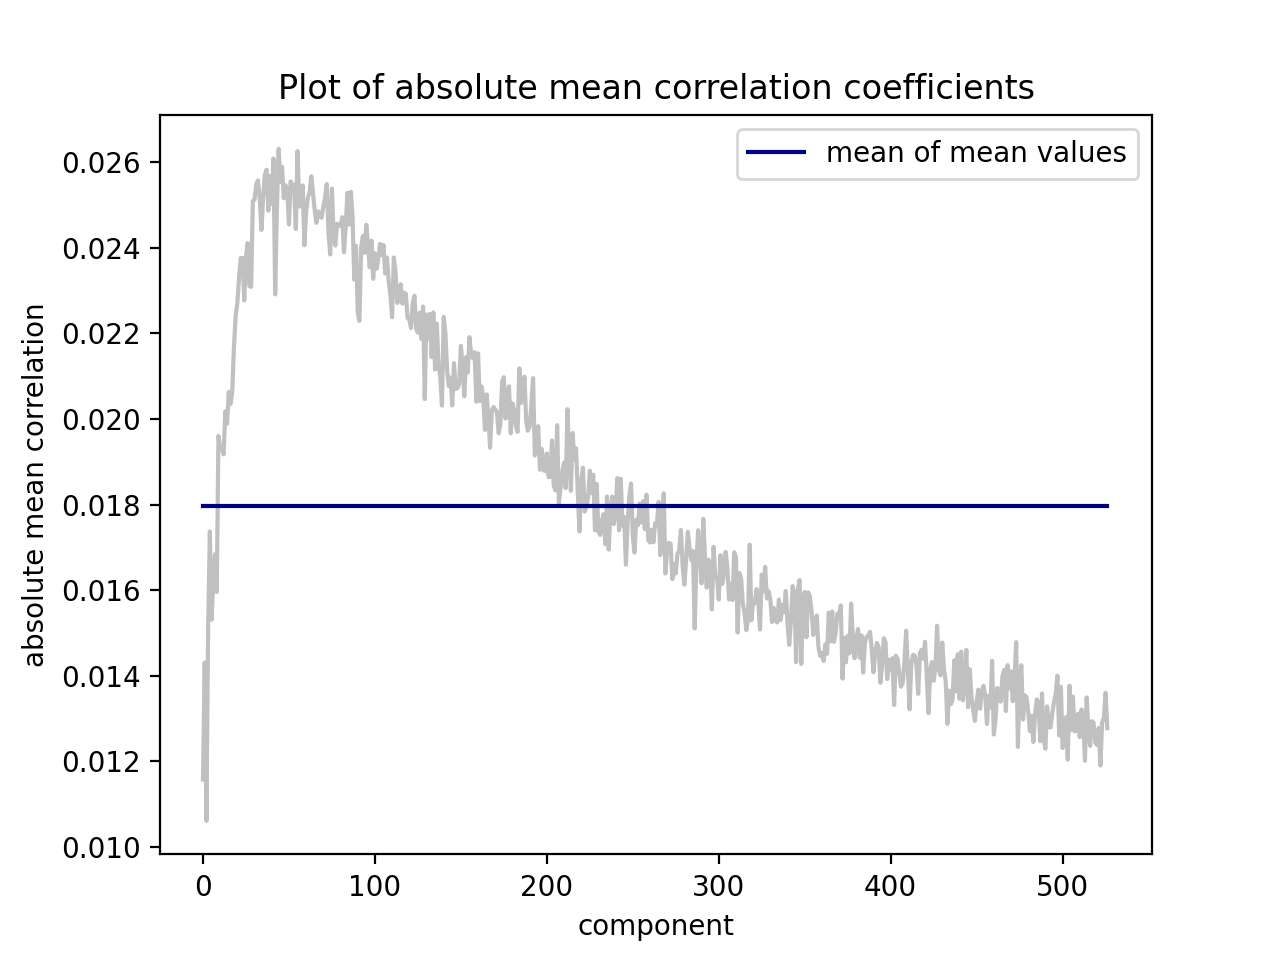
\includegraphics[scale=0.85]{validation_small_set_2_joined_PC_95_correlation_mean.png}
		\end{tabular}
		
		\caption{Plot of ESM-1b principal components' (95\%) mean and maximum correlation 
		coefficients with ProtTrans principal components (95\%)}
		\label{figure:correlationComponentsMaxAndMeanPC95}
	\end{figure}

	\newpage

	\subsection{Representation analysis}

	The first step of the analysis was to try ProtTrans embeddings 
	as input for the SLP model and compare 
	its results with the testing metrics of model trained with 
	ESM-1b. For the comparison, the primary model with ESM-1b was 
	trained again using the filtered data set. The comparison disclosed 
	that the model, which uses ProtTrans embeddings as input, performs 
	better (Table \ref{table:comparisonESMandPTmeanNormMeanJoined}).

	Out of the scope of this representation and model architecture analysis
	for binary classification, there were several attempts made to overtrain
	the classification model to predict three thermostability classes (one 
	more class was added after dividing the zero-labelled class at the temperature
	threshold of 40 degrees Celsius). The purpose of overtraining was to check 
	whether the selected architecture has a potential to be trained for the 
	multiclass classification problem. The usage of principal 
	components of protein embeddings showed that overfitting can be 
	done successfully.

	Therefore, it was decided to check whether 
	a vector of principal components could be a suitable input for the binary 
	classification task. The testing stage metrics showed worse model's performance 
	than using the original representations (Table \ref{table:comparisonESMandPTunfiltMeanPC}). 

	\begin{table}[h!]
		\caption{The comparison of scores between models trained with ESM-1b
		and ProtTrans mean representations and their principal components 
		that account for 95\% and 100\% of the unfiltered data set variance}
		\vspace{0.2cm}
		\centering
		\begin{tabular}{ | c | c c c c c c | }
			\hline 
						
			& \specialcell{Mean\\ESM-1b} & \specialcell{Mean\\ProtTrans} & \specialcell{ESM-1b\\(95\%)} & \specialcell{ProtTrans\\(95\%)} & \specialcell{ESM-1b\\(100\%)} & \specialcell{ProtTrans\\(100\%)} \\
			\hline 
			MCC & 0.843 & 0.902 & 0.699 & 0.767 & 0.698 & 0.766 \\
			Accuracy  & 0.922 & 0.951 & 0.845 & 0.880 & 0.845 & 0.879 \\
			Loss & 0.208 & 0.128 & 0.383 & 0.442 & 0.382 & 0.443 \\
			Precision & 0.919 & 0.949 & 0.910 & 0.940 & 0.909 & 0.939 \\
			Recall & 0.921 & 0.951 & 0.768 & 0.813 & 0.767 & 0.812 \\
			ROC AUC & 0.979 & 0.990 & 0.901 & 0.945 & 0.901 & 0.943 \\

			\hline    
		\end{tabular}
		\label{table:comparisonESMandPTunfiltMeanPC}
	\end{table}

	\newpage

	Before joining the embeddings, the normalisation of ESM-1b and ProtTrans 
	vectors was done. Normalised representations were taken as input to 
	the model with the same SLP architecture. For both types of embeddings 
	the results were improved (Table \ref{table:comparisonESMandPTmeanNormMeanJoined}).

	After joining ESM-1b and ProtTrans mean embeddings, an SLP was trained 
	using these joined representations. The results of this model were similar 
	to the scores of the model that was trained using only ProtTrans embeddings, 
	though the results 
	did not improve (Table \ref{table:comparisonESMandPTmeanNormMeanJoined}). 

	\begin{table}[h!]
		\caption{The comparison of testing stage scores between 
		models trained with mean, normalised mean, joined mean, 
		and normalised joined ESM-1b and ProtTrans 
		representations}
		\vspace{0.2cm}
		\centering
		\begin{tabular}{ | c | c c c c c c | }
			\hline 
						
			& ESM-1b & \specialcell{Normalised\\ESM-1b} & ProtTrans & \specialcell{Normalised\\ProtTrans} & Joined & \specialcell{Normalised\\joined} \\
			\hline 
			MCC & 0.843 & 0.858 & 0.901 & 0.915 & 0.899 & 0.920 \\
			Accuracy & 0.921 & 0.929 & 0.951 & 0.957 & 0.949 & 0.960 \\
			Loss & 0.208 & 0.248 & 0.128 & 0.143 & 0.131 & 0.139 \\
			Precision & 0.921 & 0.923 & 0.949 & 0.951 & 0.945 & 0.954 \\
			Recall & 0.917 & 0.931 & 0.949 & 0.962 & 0.951 & 0.964 \\
			ROC AUC & 0.979 & 0.982 & 0.990 & 0.991 & 0.991 & 0.992 \\
			\hline    
		\end{tabular}
		\label{table:comparisonESMandPTmeanNormMeanJoined}
	\end{table}

	\begin{figure}[!h]
		\centering
		
		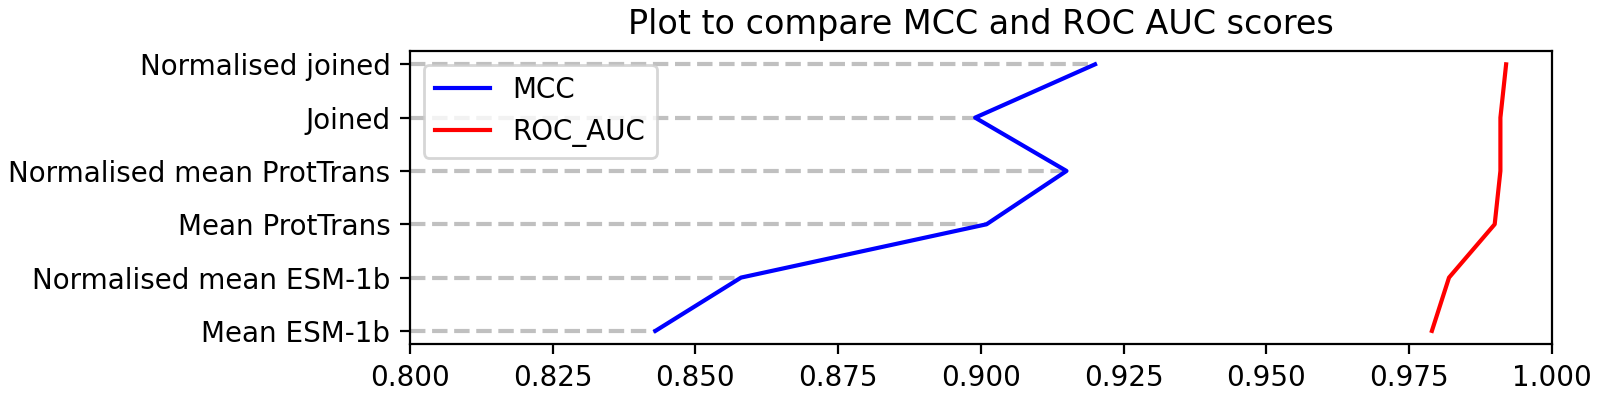
\includegraphics[scale=0.65]{ESM_PT_comparison_MCC_ROC_scores.png}
		
		\caption{Comparison of SLP models', which were trained with mean and 
		normalised mean ESM-1b, ProtTrans, and joined representations, MCC 
		and ROC AUC scores}
		\label{figure:MCC_ROCscores_ESMandPT}
	\end{figure}

	However, joining the normalised ESM-1b and ProtTrans mean representations 
	showed the best results. Since joined representations require
	generation of ESM-1b embeddings, this type of representation does not 
	solve the length limitation problem that was noticed in the previous work. 
	Nevertheless, slightly improved results can be observed when normalised 
	representations are used, the process of normalisation depends on the data 
	set, which is not convenient in the process of development until the 
	final data set is established. Therefore, the optimal choice for 
	this stage of development was mean ProtTrans embeddings.

	Nonetheless, ProtTrans already demonstrated the impact for the 
	model's improvement on the performance, it was decided to finish up 
	the different representation and architecture analysis using embeddings
	of both protein language models for completeness. The results 
	of the consequent analysis 
	did not change the conclusion regarding ProtTrans influence for the 
	results using any variation of analysed representations (listed in the
	section \ref{analysedRepresentations}) - in all cases the model that took 
	ProtTrans embeddings as input performed significantly better (Figure 
	\ref{figure:scoresRepresentationsESMandPT}).

	\begin{figure}[h!]
		\centering
		\begin{tabular}{@{}c@{}}
			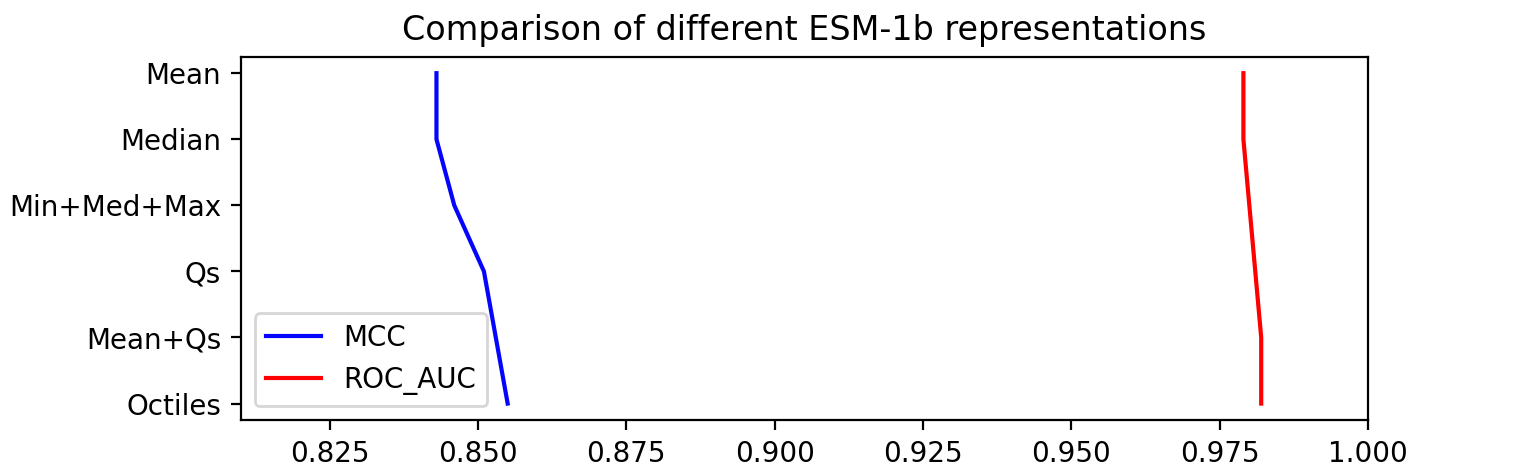
\includegraphics[scale=0.7]{SLP_ESM_003_diff_representations.png}
		\end{tabular}

		\begin{tabular}{@{}c@{}}
			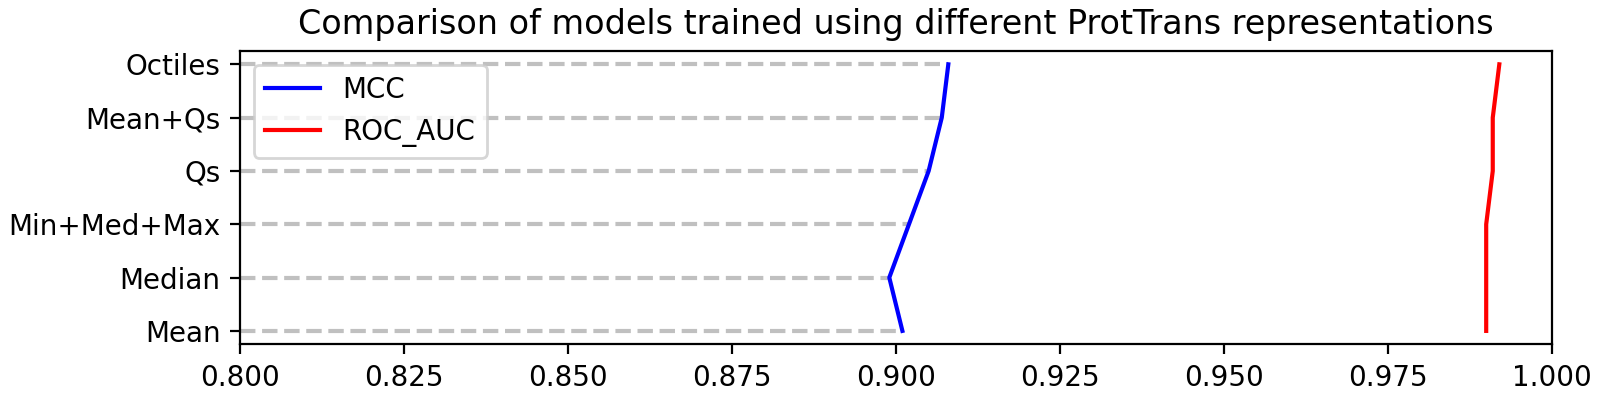
\includegraphics[scale=0.7]{SLP_PT_003_diff_representations.png}
		\end{tabular}
		
		\caption{Comparison of SLP models', which were trained with different
		ESM-1b and ProtTrans representations, MCC and ROC AUC scores}
		\label{figure:scoresRepresentationsESMandPT}
	\end{figure}

	\newpage

	\subsection{Architecture analysis}

	The final stage of work was to analyse, which architecture of the
	model gives the best prediction results.

	The results of SLP models were compared with the new models 
	trained with mean embeddings of ESM-1b and ProtTrans (Figure 
	\ref{figure:scoresMLP_ESMandPT}). Models with 
	hidden layers reached achieved results than the single-layer 
	models: the best model that used ProtTrans embeddings reached
	MCC of 0.916, meanwhile the SLP using ProtTrans embeddings 
	reached MCC of 0.901, although the training duration was 9 times 
	longer.

	\begin{figure}[h!]
		\centering
		\begin{tabular}{@{}c@{}}
			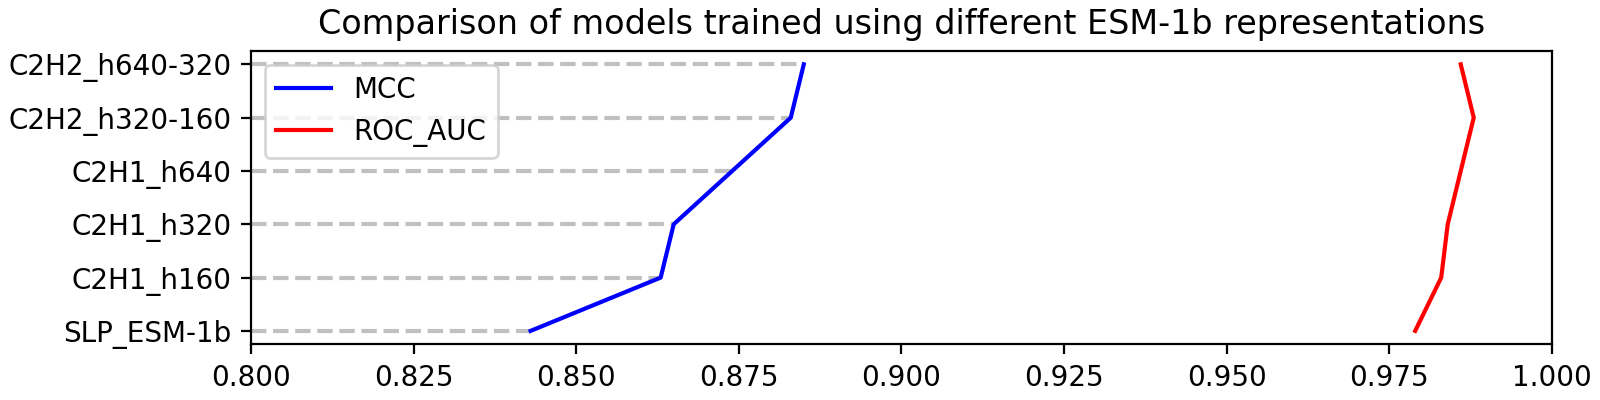
\includegraphics[scale=0.6]{MLP_ESM.png}
		\end{tabular}

		\begin{tabular}{@{}c@{}}
			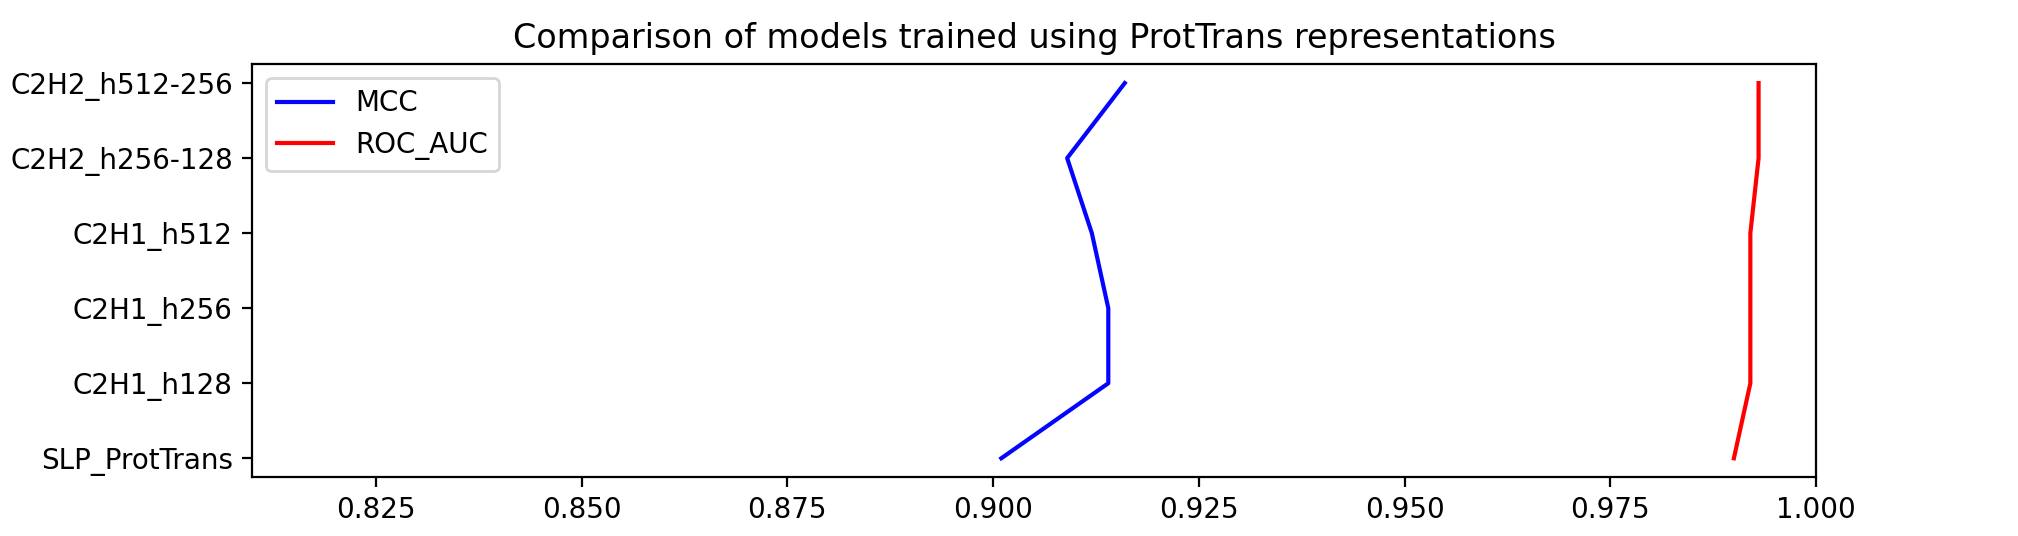
\includegraphics[scale=0.6]{MLP_PT.png}
		\end{tabular}
		
		\caption{Comparison of different architecture models', which were trained using 
		ESM-1b or ProtTrans embeddings, MCC and ROC AUC scores}
		\label{figure:scoresMLP_ESMandPT}
	\end{figure}

	\newpage

	\section{Conclusions}

	The results of this work provided following conclusions: for 
	further development of the final method ProtTrans mean and 
	octiles embeddings will be used. Nevertheless, models that used 
	mean ProtTrans embeddings did not provide as good results as 
	the octiles representations in this work, due to more efficient 
	training 
	procedure with mean embeddings, both these representations will 
	be used for the further development of the tool.
	
	Additionally, this work 
	showed that it is worth to use the model's architecture with 
	two hidden layers with sizes 512 and 256.

	\begin{table}[h!]
		\caption{The comparison of testing stage scores between SLP
		models trained with mean, normalised mean, and octiles ProtTrans
		representations and model's with 2 hidden layers trained with 
		mean ProtTrans representations}
		\vspace{0.2cm}
		\centering
		\begin{tabular}{ | c | c c c c | }
			\hline 
						
			& Mean (SLP) & \specialcell{Normalised \\mean (SLP)} & Octiles (SLP) & \specialcell{Mean \\ (MLP h512-256)} \\
			\hline 
			MCC & 0.901 & 0.915 & 0.910 & 0.919 \\
			Accuracy & 0.951 & 0.957 & 0.955 & 0.960 \\
			Loss & 0.128 & 0.143 & 0.125 & 0.192 \\
			Precision & 0.949 & 0.951 & 0.959 & 0.954 \\
			Recall & 0.949 & 0.962 & 0.947 & 0.963 \\
			ROC AUC & 0.990 & 0.991 & 0.992 & 0.993 \\
			\hline    
		\end{tabular}
		\label{table:conclusionsTable}
	\end{table}

	\begin{figure}[h!]
		\centering
		
		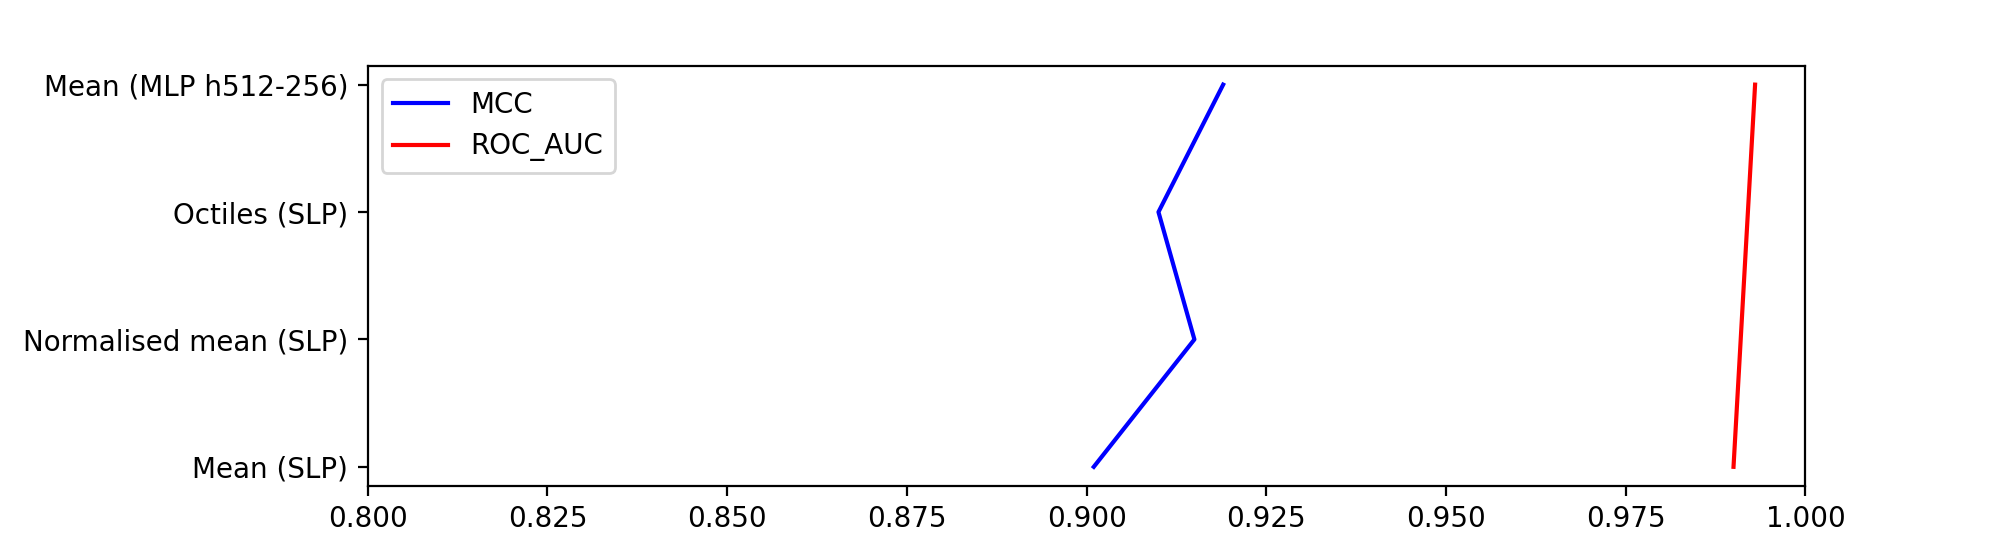
\includegraphics[scale=0.6]{conclusions_plot.png}
		
		\caption{Comparison of different models', which were trained using 
		ProtTrans embeddings, MCC and ROC AUC scores}
		\label{figure:conclusionsPlot}
	\end{figure}

	The next steps of the development will be to generate the 
	mentioned representations for the bigger data set, which 
	will be used to train the binary classification model with 
	the architecture of two hidden layers.

	\section{Availability}

	The code that was used to receive the results of this work can be found
	in the designated Github repository: 
	\href{https://github.com/ievapudz/Course_Work_Project}{https://github.com/ievapudz/Course\_Work\_Project}.

	\newpage

	\section{Abstract in Lithuanian (Santrauka)}

	\begin{otherlanguage}{lithuanian}
	
    Šis darbas yra ankstesnio darbo - binarinę baltymų klasifikaciją 
    pagal termostabilumą vykdančio modelio vystymo - tęsinys. Vystomas
    modelis buvo vieno sluoksnio perceptronas, kurio įvestis ESM-1b 
	\cite{rives2021biological}
    baltymų kalbos modelio generuojamos skaitinės reprezentacijos, o
    išvestis - prognozė kiekvienam baltymui, kaip tikėtina, kad jis 
    priklauso termostabilių baltymų klasei.
    
    Termostabilumo klasės buvo atskirtos 65 Celsijaus laipsnių riba:
    baltymai, kurie yra stabilūs žemesnėje nei nurodyta riba 
    temperatūroje, priskiriami klasei su žyme '0', o stabilūs 
    baltymai 65 laipsnių ir aukštesnėje temperatūroje yra 
    laikomi klasės '1' nariais.
    
    Minėtas klasifikatorius buvo apmokytas naudojant duomenų rinkinį, 
	kuriame
    saugomos organizmų augimo temperatūros 
	\cite{engqvist_martin_karl_magnus_2018_1175609}. Į duomenų rinkinį 
	taip pat
    buvo įtraukti organizmų proteomų identifikatoriai, kurie buvo
    panaudoti surinkti proteomui priklausančius baltymus ir juos 
    sužymėti pagal organizmo augimo temperatūrą.

    Nepaisant to, kad klasifikatorius pateikė neblogus rezultatus,
    testuojant metodą išryškėjo svarbus trūkumas. Kadangi ESM-1b
    skaitinių reprezentacijų kūrimas buvo apribotas baltymo ilgiu,
    nebuvo galima sugeneruoti reprezentacijų baltymams, kurie buvo 
    ilgesni nei 1022 aminorūgštys. Dėl šios priežasties buvo nutarta
    išmėginti ProtTrans \cite{elnaggar2020prottrans} skaitines 
	reprezentacijas kaip klasifikatoriaus
    įvestį, nes šis baltymų kalbos modelis buvo apmokytas be apribojimo 
    baltymo ilgiui. 

    Taip pat domino išmėginti ne tik suvidurkintas skaitines 
    reprezentacijas, bet ir išnaudoti galimybę išgauti kitaip
    apibendrintas kiekvienos aminorūgšties reprezentacijas bei 
    patikrinti, ar gauti kitokie įvesties vektoriai suteikia
    geresnius rezultatus. 
  
    Apart reprezentacijų analizės, taip pat buvo atlikti 
	eksperimentai
    patikrinimui, ar kitokios modelių architektūros turės
    ženklios įtakos modelio veikimui.

	Šios analizės rezultatai parodė, kad geriausia naudoti ProtTrans
	vidurkių bei oktilių skaitines reprezentacijas, kol bus nustatytas 
	galutinis duomenų rinkinys modelio apmokymui. Taip pat remiantis
	gautais rezultatais galima teigti, kad geriausia modelio 
	architektūra baltymų klasifikavimo pagal termostabilumą problemos
	sprendimui yra neuroninio tinklo modelis su dviem paslėptais
	sluoksniais.
      
    Gautos analizių išvados suteiks naudingų įžvalgų galutinio
    metodo baltymų klasifikacijai pagal termostabilumą apibrėžimui.

	\end{otherlanguage}

	\newpage
	
	\nocite{*}
	
	\normalsize

\bibliography{references} 
\bibliographystyle{ieeetr}

\end{document}
